\chapter{Smart Contract ed Ethereum}

L'idea fondamentale degli \textbf{smart contract} (concetto introdotto da Nick Szabo negli anni '90) nasce dalla volontà di superare i limiti strutturali dei contratti tradizionali, spesso definiti in modo provocatorio \textit{dumb contracts}. A differenza di un contratto legale che richiede la redazione di un avvocato, dipende dalla giurisdizione statale e necessita di interpretazione umana, uno smart contract è un protocollo informatico. 

Esso presenta tre caratteristiche distintive:
\begin{itemize}
    \item \textbf{Assenza di ambiguità}: Essendo scritto in codice deterministico, il contratto esegue esattamente ciò che è stato programmato, riducendo i margini di interpretazione.
    \item \textbf{Auto-esecuzione}: Non necessita di intermediari (come giudici o notai) per essere applicato; la piattaforma di esecuzione ne garantisce l'adempimento forzoso.
    \item \textbf{Trasparenza}: Il codice è pubblico, verificabile da chiunque e memorizzato in modo immutabile sulla blockchain.
\end{itemize}

\section{Limitazioni di Bitcoin Script}
Bitcoin possiede un linguaggio di scripting interno (\textbf{Script}), progettato però per essere intenzionalmente limitato per ragioni di sicurezza. I suoi principali vincoli sono:
\begin{itemize}
    \item \textbf{Logica limitata}: Script non è \textit{Turing-complete}. Supporta principalmente operazioni di accettazione o rifiuto di transazioni (\textit{stateless logic}).
    \item \textbf{Assenza di loop}: Per evitare attacchi \textit{Denial of Service} (DoS) basati su cicli infiniti, non sono ammesse istruzioni di iterazione.
    \item \textbf{Mancanza di stato}: Lo script non ha memoria persistente se non lo stack temporaneo di esecuzione; non può "ricordare" dati tra una transazione e l'altra.
    \item \textbf{Blockchain Blindness}: Lo script è ``cieco'' rispetto ai dati ambientali della blockchain (come timestamp o difficoltà), limitandosi a verificare le condizioni di sblocco degli UTXO.
\end{itemize}
Queste restrizioni, insieme all'uso di una \textbf{whitelist} di script standard accettati dai miner, rendono Bitcoin un sistema eccellente per il trasferimento di valore, ma inadatto a eseguire programmi complessi.

\subsection{Il Caso Namecoin: Limiti della Logica di Bitcoin}

Per comprendere appieno le limitazioni di Bitcoin Script, è utile analizzare il caso di \textbf{Namecoin}, il primo progetto che ha tentato di implementare un sistema DNS (Domain Name System) decentralizzato sulla blockchain. L'obiettivo era creare un mapping immutabile del tipo:
\[ \text{Domain Name} \longrightarrow \text{IP Address} \]

Un sistema di questo tipo richiederebbe il supporto per tre operazioni fondamentali:
\begin{itemize}
    \item \texttt{NameCoin.register(ownerAddr, domainName, initialVal)}: operazione per la registrazione iniziale di un dominio non ancora censito.
    \item \texttt{NameCoin.update(domainName, newVal, newOwner, ownerSig)}: operazione per aggiornare l'indirizzo IP associato o trasferire la proprietà del dominio. Quest'ultima richiede necessariamente la firma crittografica del proprietario attuale (\textit{ownerSig}).
    \item \texttt{NameCoin.lookup(domainName)}: funzione di sola lettura, accessibile a chiunque, per risolvere il nome di dominio nel rispettivo indirizzo IP.
\end{itemize}

In linea teorica, si potrebbe tentare di implementare questa logica in Bitcoin estendendo la \textbf{ScriptPubKey} con nuovi comandi, salvando all'interno dell'UTXO la coppia (dominio, IP) e vincolando la spesa alla verifica della chiave pubblica del proprietario.
\begin{figure}[H]
    \centering
    
\includegraphics[width=0.3\linewidth]{Images/capitolo_mdr_3/namecoin_script.png}
\end{figure}
Tuttavia, emerge un limite tecnico insormontabile: \textbf{Bitcoin Script non può verificare se un dominio sia già stato registrato}. Poiché ogni script viene eseguito in isolamento e ha accesso solo ai dati della transazione corrente (proprietà \textit{stateless}), non può interrogare l'intero set di UTXO per convalidare la policy di unicità del nome (fondamentale per un DNS). 


A causa di questa incapacità di gestire uno stato globale condiviso, l'idea non ha potuto trovare spazio nel protocollo Bitcoin originale. Namecoin è stato quindi costretto a implementare un \textbf{hard fork}, dando vita a una nuova criptovaluta indipendente. Questo ha comportato la necessità di un nuovo processo di \textit{bootstrap} per creare una community e attirare potenza di calcolo dedicata, frammentando di fatto l'ecosistema invece di integrarsi in esso.

\section{La Piattaforma Ethereum}
Ethereum nasce con l'obiettivo di superare queste barriere, fornendo uno strato computazionale universale sopra la blockchain. Questo ha permesso la nascita di ecosistemi complessi come gli \textbf{NFT}, la finanza decentralizzata (\textbf{DeFi}), il \textbf{gaming on-chain} e le organizzazioni autonome (\textbf{DAO}).

A differenza di Bitcoin, basato sul modello UTXO (un insieme di "monete" non spese), Ethereum utilizza un \textbf{Account-based model}. La blockchain non è solo una lista di transazioni, ma una \textbf{transizione di stati} che modifica costantemente il \textbf{World State} (lo stato globale del network).

\subsection{L'unità monetaria: Ether}
Il valore all'interno della rete è denominato in \textbf{Ether} (ETH). Sebbene l'utente medio ragioni in ETH, internamente il sistema opera esclusivamente in \textbf{Wei}, la minima unità divisibile:
\begin{itemize}
    \item 1 Ether = $10^{18}$ Wei
    \item 1 Finney = $10^{15}$ Wei ($10^{-3}$ ETH)
    \item 1 Szabo = $10^{12}$ Wei ($10^{-6}$ ETH)
\end{itemize}

\subsection{Consenso: dal PoW al Proof of Stake}
Dalla genesi fino a settembre 2022 (evento noto come \textbf{The Merge}), Ethereum ha utilizzato la Proof of Work (basata sull'algoritmo \textit{Ethash}). Per prevenire il dominio degli ASIC, l'algoritmo era stato progettato per essere \textit{memory-hard}, favorendo il mining tramite GPU.

Il passaggio alla \textbf{Proof of Stake} era previsto fin dal design iniziale. Per forzare la migrazione e disincentivare i miner a restare sulla vecchia catena, è stata introdotta la \textbf{Difficulty Bomb} un meccanismo che aumenta esponenzialmente la difficoltà del puzzle crittografico fino a rendere impossibile la produzione di blocchi, rendendo la rete PoW di fatto inutilizzabile e accelerando la transizione verso il nuovo modello basato sullo \textit{staking}.

A differenza di Bitcoin, dove il tempo tra i blocchi è di 10 minuti, Ethereum produce un blocco (o \textit{slot}) ogni 12 secondi, garantendo una finalità delle transazioni molto più rapida. Inoltre, l'emissione di ETH non ha un tetto massimo fisso di 21 milioni, ma è regolata da meccanismi di \textit{burn} e ricompense per i validatori che bilanciano inflazione e deflazione.


\subsection{Tipologie di Account}
In Ethereum esistono due tipi di account, entrambi identificati da un indirizzo e dotati di un bilancio in Ether:
\begin{itemize}
    \item \textbf{Externally Owned Accounts (EOA)}: Controllati da utenti umani tramite chiavi private e firme ECDSA. Possono inviare transazioni per trasferire ETH o interagire con i contratti.
    \item \textbf{Contract Accounts}: Account governati esclusivamente dal loro codice (\textbf{EVM Bytecode}). Non possiedono chiavi private e le loro azioni sono innescate solo se ricevono una transazione da un EOA o da un altro contratto. Il codice di un contratto è \textbf{immutabile}; per aggiornarlo, gli sviluppatori utilizzano spesso il pattern \textit{Proxy}, che permette di puntare l'indirizzo del contratto a una nuova logica in modo trasparente.
\end{itemize}
\begin{figure}[H]
    \centering
    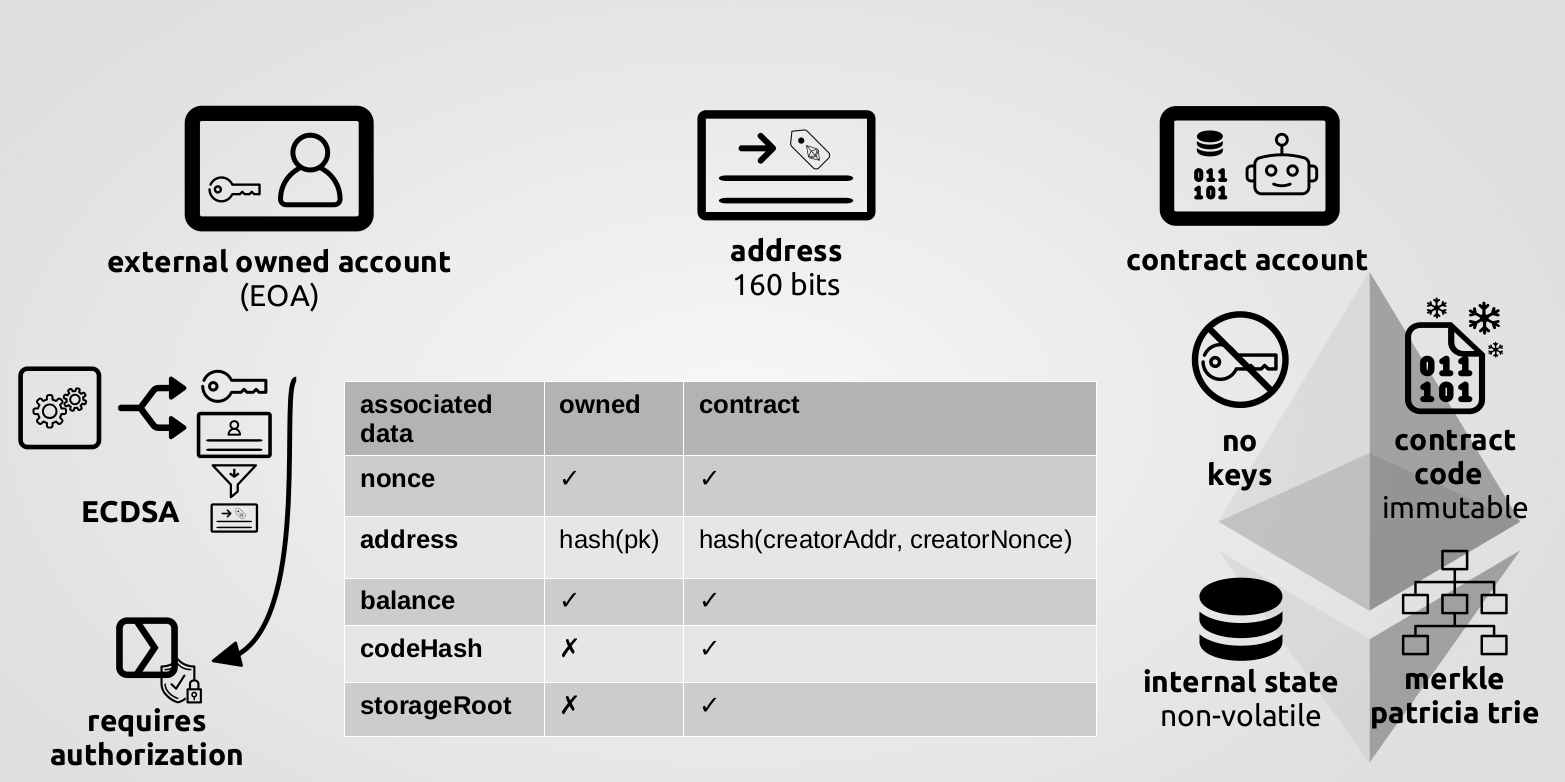
\includegraphics[width=0.8\linewidth]{Images/capitolo_mdr_3/contract_account_vs_eoa.png}
\end{figure}

Analizziamo adesso uno per uno i dati degli account:
\begin{itemize}
    \item \textbf{Nonce}: La nonce negli account rappresenta un numero che serve a prevenire gli attacchi di replay. La firma di ogni transazione, infatti, oltre che i dati contiene anche questa nonce che, subito dopo la firma, viene aggiornata di uno. La firma viene considerata valida solo se la nonce nella transazione corrisponde a quelle dell'account segnata in quel momento nel world state. In Bitcoin ricordiamo che non è effettivamente presente una nonce per prevenire attacchi di replay, tuttavia, gli uTXO se vogliamo possono fungere come una sorta di Nonce perché sono spendibili solo una volta. 
    Nei contratti, la nonce serve a contare quanti contratti sono stati creati a partire da quel contratto ma questa funzione la vedremo dopo nel dettaglio.
    \item \textbf{Indirizzo}: Conosciamo già l'importanza degli indirizzi nel sistema blockchain per riferirci ad uno specifico account. Per quanto riguarda gli EOA, questo è banalmente l'hash della chiave pubblica mentre, per quanto riguarda i contratti questo è l'hash dell'indirizzo del creatore insieme alla sua nonce. Ricordiamo che per creatore di un contratto possiamo anche avere altri contratti.
    \item \textbf{Balance}: Come abbiamo già detto, sia gli EOA che i contratti possono possedere un bilancio per effettuare transazioni o attivare altri contratti.
    \item \textbf{CodeHash}: Il CodeHash è un campo posseduto solo dai contratti. Poiché il codice del contratto è salvato nella blockchain, che possiamo immaginare come una sorta di database, possiamo dire che il CodeHash funge da ID per cercare e trovare velocemente il codice.
    \item \textbf{StorageRoot}: Ogni contratto possiede una certa memoria che gli servirà per mantenere al suo interno uno stato non volatile. Questa è memorizzata sotto forma di \textbf{Merkle Patricia Trie} che descriveremo tra poco. Nello specifico, anche in questo caso lo StorageRoot è la radice di questo albero che servirà per effettuare prove di appartenenza.
\end{itemize}


\subsection{Merkle Patricia Trie (MPT)}
I \textbf{Merkle Patricia Trie} rappresentano la struttura dati fondamentale su cui poggia l'architettura di Ethereum, utilizzati sia per la gestione del \textbf{World State} (lo stato globale di tutti gli account) che per lo \textbf{storage dei singoli contratti}.

Essi nascono come un'integrazione tra i \textit{Patricia Trie} (noti anche come \textit{Radix Tree}) e la logica crittografica dei \textit{Merkle Tree}:

\begin{itemize}
    \item \textbf{Struttura Patricia (Radix Tree)}: Implementano una mappa $key \to value$ dove la chiave (solitamente una stringa esadecimale derivata da un hash) viene utilizzata per navigare l'albero. Il vantaggio principale è la condivisione dei prefissi: chiavi simili condividono lo stesso percorso iniziale, riducendo drasticamente la ridondanza e lo spazio di archiviazione. Se una chiave non è presente, il percorso si interrompe restituendo un valore nullo.
    
    \item \textbf{Componente Merkle}: Ogni nodo dell'albero è identificato dall'hash dei suoi contenuti (e dei puntatori ai suoi figli). Questo trasforma l'intera struttura in un \textbf{commitment crittografico}: la radice (\textit{Root Hash}) è un'impronta digitale unica di tutto lo stato. Ciò permette di generare \textbf{Proof of Membership} (o prove di Merkle), consentendo ai nodi leggeri di verificare l'esistenza e il valore di un dato senza possedere l'intero database.
\end{itemize}

\begin{figure}[H]
    \centering
    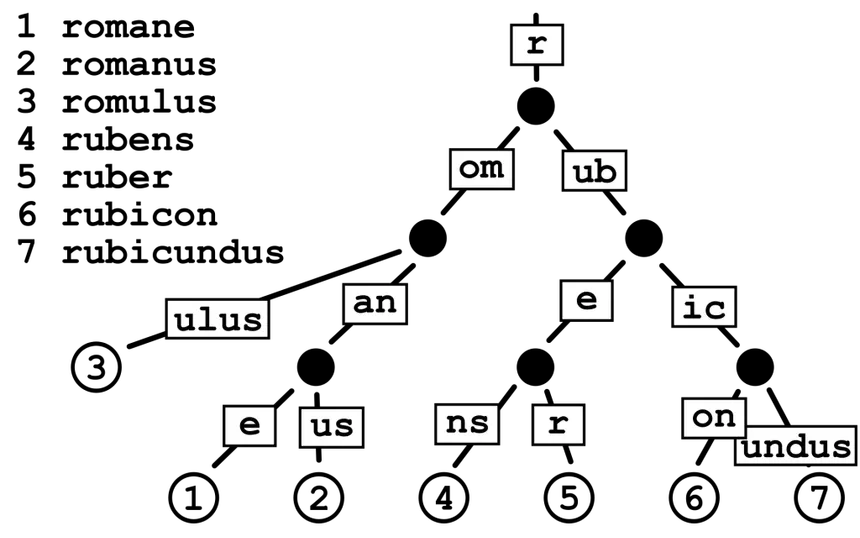
\includegraphics[width=0.7\linewidth]{Images/capitolo_mdr_3/radix_tree.png}
\end{figure}

A differenza di un semplice Merkle Tree statico (come quello usato nei blocchi di Bitcoin), l'MPT è una \textbf{struttura dinamica}. È progettato per gestire inserimenti, modifiche e cancellazioni frequenti in modo efficiente: 
\begin{itemize}
    \item Quando un valore viene aggiornato (ad esempio il bilancio di un account), è necessario ricalcolare solo gli hash dei nodi lungo il percorso che va dalla foglia modificata fino alla radice.
    \item In un albero bilanciato, la complessità di queste operazioni è logaritmica rispetto al numero di elementi, garantendo prestazioni elevate anche con milioni di account.
\end{itemize}

\subsection{World State}
Il \textbf{World State} rappresenta lo stato globale e aggiornato dell'intero ecosistema Ethereum. Tecnicamente, è implementato come un \textbf{Merkle Patricia Trie} (MPT) la cui radice (\textit{State Root}) è inclusa in ogni blocco della blockchain. 

Questo archivio può essere visualizzato come un database chiave-valore dove:
\begin{itemize}
    \item \textbf{Chiave}: L'indirizzo esadecimale di 20 byte dell'account (previa applicazione di un hash per bilanciare l'albero).
    \item \textbf{Valore}: Lo stato dell'account serializzato, che comprende \textit{nonce}, \textit{balance}, \textit{storageRoot} e \textit{codeHash}.
\end{itemize}

Grazie alla struttura MPT, è possibile fornire una \textbf{Proof of Membership} per dimostrare l'esistenza e il saldo di un account senza dover scansionare l'intera rete.

Per ogni contratto esiste un ulteriore \textbf{Storage Trie}. Qui vengono mappate chiavi di 256 bit (derivanti spesso dalla posizione o dal nome della variabile nel codice Solidity) in valori di 256 bit. 

Se una variabile viene dichiarata ma mai inizializzata, o se viene esplicitamente posta uguale a \texttt{0}, l'MPT non memorizza alcun nodo per quella chiave. 
Di conseguenza, una ricerca per una chiave inesistente restituisce sempre \texttt{0}, permettendo un risparmio considerevole di spazio poiché si memorizzano solo i valori non nulli.

Per poter inserire un oggetto complesso come un account (composto da 4 campi distinti) all'interno di un nodo dell'albero di Merkle, è necessario prima trasformarlo in una sequenza di byte "piatta". Ethereum utilizza a questo scopo lo standard \textbf{RLP}.

L'RLP è il sistema di serializzazione primario di Ethereum che serve a codificare strutture dati (liste, stringhe, interi) in un formato binario compatto.

\subsection{Transazioni}
In Ethereum esistono le classiche transazioni che abbiamo già visto in Bitcoin che possono essere effettuate solo da EOA. Queste contengono al loro interno:
Ogni transazione contiene i seguenti campi fondamentali:
\begin{itemize}
    \item \textbf{Nonce}: Un contatore che indica quante transazioni sono state inviate dall'indirizzo mittente. Serve a garantire l'ordine di esecuzione e a prevenire attacchi di \textit{replay}.
    \item \textbf{Recipient (to)}: L'indirizzo di 20 byte del destinatario. Se il campo è vuoto (nullo), la transazione viene interpretata come una creazione di contratto.
    \item \textbf{Value}: L'ammontare di Ether (espresso in \textit{Wei}) da trasferire dal mittente al destinatario.
    \item \textbf{Gas Limit}: La quantità massima di unità di gas che il mittente è disposto a consumare per l'esecuzione.
    \item \textbf{Gas Price}: Il prezzo (in Wei) che il mittente è disposto a pagare per ogni unità di gas consumata.
    \item \textbf{Data (o Input)}: Un campo di lunghezza variabile che contiene i dati necessari per l'attivazione di funzioni nei contratti o il codice di inizializzazione per i nuovi contratti.
    \item \textbf{Firma ECDSA (v, r, s)}: Ethereum utilizza una variante di ECDSA chiamata \textbf{public key recovery}. Invece di includere esplicitamente il campo \textit{from} (mittente), il protocollo estrae la chiave pubblica (e quindi l'indirizzo) direttamente dalla firma e dal messaggio transazionale, ottimizzando lo spazio nella blockchain.
\end{itemize}
Queste transazioni possono essere di vari tipi:
\begin{itemize}
    \item \textbf{Currency Transfer:} Questa è la classica transazione in cui un EOA invia dei soldi ad un altro EOA.
    \item \textbf{Contract Activation:} Tramite questo tipo di transazione è possibile attivare una funzione di un contratto. I contratti, infatti, metteranno a disposizione proprio delle funzioni che potranno prendere in input anche dei dati sul quale lavorare.
    \item \textbf{Contract Creation:} Questa transazione viene fatta verso un indirizzo nullo con una certa semantica e servirà alla generazione di un nuovo contratto. Tra questi valori sarà presente l'init che sarà un codice che, una volta eseguito, produrrà il codice reale del contratto.
\end{itemize}
\begin{figure}[H]
    \centering
    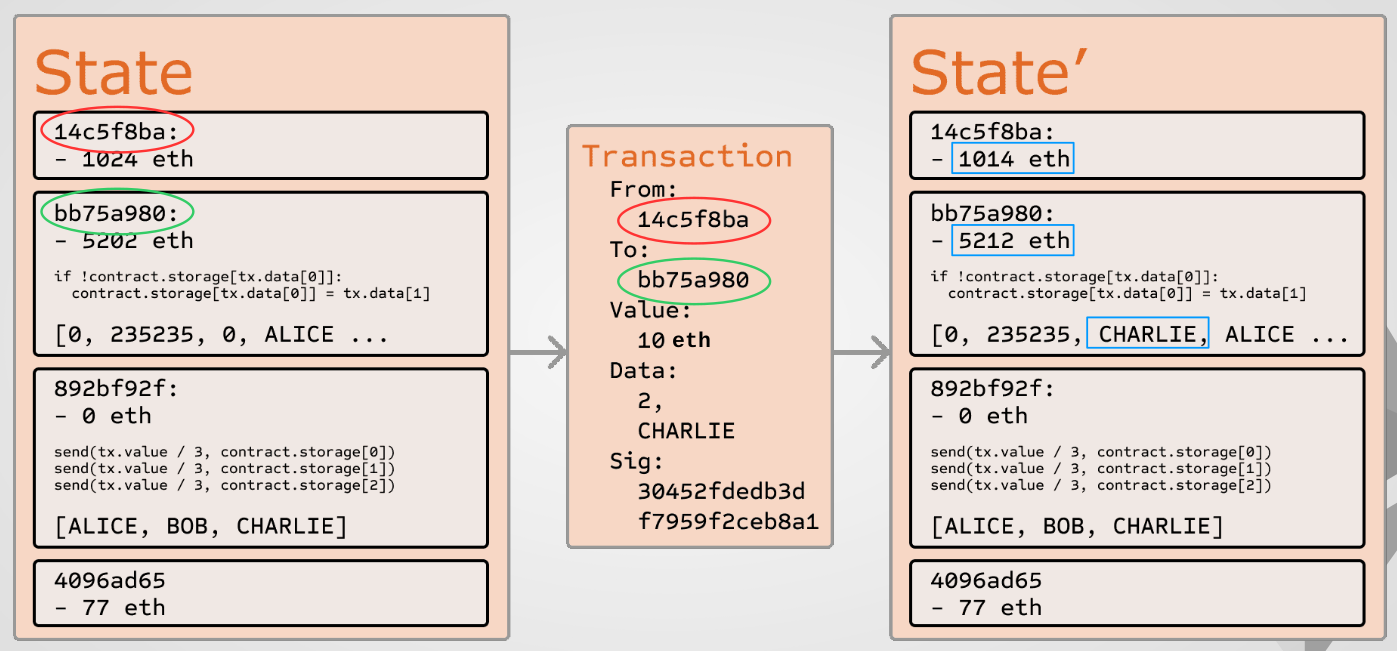
\includegraphics[width=0.7\linewidth]{Images/capitolo_mdr_3/simple_transaction.png}
\end{figure}

\subsection{Messaggi}

Mentre le transazioni sono originate esclusivamente da account esterni (EOA), i contratti interagiscono tra loro attraverso i \textbf{messaggi}, spesso definiti \textbf{transazioni interne}. 

Sebbene un messaggio sia concettualmente simile a una transazione (possiede un mittente, un destinatario, un valore e dei dati), presenta una differenza fondamentale: \textbf{non richiede una firma digitale}.

La sicurezza e l'autorizzazione nei messaggi non derivano dalla crittografia a chiave pubblica, ma dalla logica deterministica della \textit{Ethereum Virtual Machine} (EVM):
\begin{itemize}
    \item \textbf{Catena di Fiducia}: Ogni messaggio è l'effetto di una transazione originale firmata da un EOA. Se l'utente $A$ firma una transazione per il Contratto $B$, e il codice di $B$ prevede l'invio di un messaggio al Contratto $C$, l'intero processo è autorizzato dalla firma iniziale di $A$.
    \item \textbf{Assenza di Chiavi}: I contratti non possiedono una chiave privata. La loro "volontà" è espressa esclusivamente dal codice immutabile memorizzato sulla blockchain. È il protocollo stesso a garantire che il campo \texttt{msg.sender} (il mittente del messaggio) corrisponda effettivamente all'indirizzo del contratto che ha generato la chiamata.
\end{itemize}

Esattamente come per le transazioni, possiamo distinguere tre operazioni principali eseguite tramite messaggi:
\begin{itemize}
    \item \textbf{Currency Transfer}: Un contratto trasferisce una parte del proprio bilancio in Ether a un EOA o a un altro contratto (solitamente tramite le istruzioni \texttt{transfer} o \texttt{call}).
    \item \textbf{Contract Activation (Message Call)}: Un contratto chiama una funzione di un altro contratto, passando dei parametri e attendendo eventualmente un valore di ritorno.
    \item \textbf{Contract Creation}: Un contratto genera un nuovo contratto "figlio" utilizzando l'istruzione \texttt{CREATE} o \texttt{CREATE2}. In questo caso, l'indirizzo del nuovo contratto sarà derivato dall'indirizzo del contratto "padre" e dalla sua \textit{nonce}.
\end{itemize}
\subsection{Block Building}
Il processo di creazione e validazione dei blocchi di Ethereum rappresenta una delle più grandi differenze rispetto al sistema Bitcoin. Ethereum, infatti, dopo un periodo iniziale basato sulla Proof-of-Work, ha abbandonato questo meccanismo per passare a un sistema chiamato Proof-of-Stake (PoS).

L'idea di fondo è quella di evitare l'eccessivo consumo elettrico causato dalla risoluzione dell'hash puzzle; al suo posto, viene utilizzato un sistema in cui i partecipanti mettono a disposizione il cosiddetto stake, ovvero una quota dei propri possedimenti in criptovaluta (Ether) bloccata come deposito di garanzia. Un validatore che propone o attesta un blocco non valido, o che tenta di frodare la rete, viene penalizzato attraverso il meccanismo di \textbf{slashing}, che comporta la distruzione di una parte o della totalità del patrimonio depositato. Il processo di costruzione e validazione di un blocco avviene come segue:
\begin{enumerate}
    \item Raccolta delle transazioni: Il validatore selezionato per il turno corrente (chiamato Block Proposer) raccoglie una serie di transazioni $TX_0, \dots, TX_{n-1}$ dalla mempool (la vasca di memoria in cui sostano le transazioni in attesa).
    \item Esecuzione e calcolo dello stato: Vengono eseguite le transazioni all'interno della Ethereum Virtual Machine (EVM), modificando i saldi dei conti ed eseguendo il codice degli smart contract coinvolti. Vengono calcolate le commissioni e, infine, viene generato il nuovo stato globale della rete, noto come world state.
    \item Propagazione e validazione (Attestazione): Il blocco appena creato viene propagato nella rete. Un comitato di altri validatori (chiamati Attesters) verifica l'integrità e la correttezza del blocco. Se il blocco è valido, i validatori inviano la propria approvazione (attestation). Nel caso in cui un validatore dovesse attestare come valido un blocco che non lo è, verrebbe penalizzato con la perdita del proprio deposito.
\end{enumerate}
Per poter essere scelti, i validatori devono aver depositato (messo in stake) esattamente 32 ETH. Più nodi validatori un utente possiede (ognuno con 32 ETH), maggiori sono le sue probabilità complessive di essere estratto. All'inizio di ogni epoca, il protocollo utilizza l'algoritmo RANDAO per generare un numero casuale condiviso e sicuro. Questo numero serve a estrarre a sorte, dall'intero pool globale, i 32 Block Proposers (uno per ogni slot dell'imminente epoca) e a formare i comitati di validatori (Attesters) che dovranno votare quei blocchi.
\subsubsection{Struttura dei Blocchi}
La struttura dei blocchi Ethereum codifica tutte le informazioni necessarie per la validazione e l’incorporazione di questi nella blockchain.
\begin{figure}[H]
    \centering
    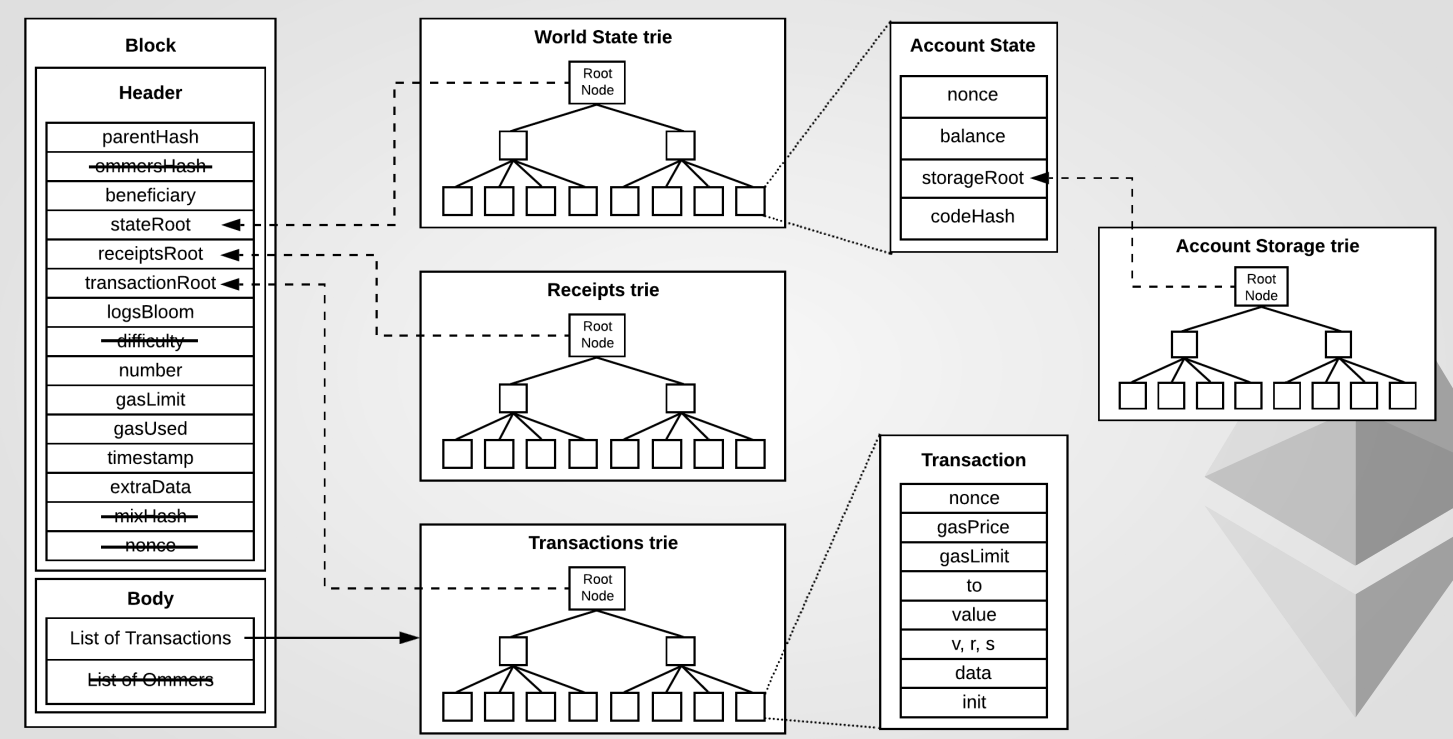
\includegraphics[width=0.7\linewidth]{Images/capitolo_mdr_3/blocco_eth.png}
\end{figure}
Un blocco è composto principalmente da due componenti:
\begin{itemize}
    \item \textbf{Header}: Questo contiene i metadati essenziali a rappresentare i vari stati. Tra questi troviamo:
    \begin{itemize}
        \item \textbf{parentHash:} L'hash Keccak a 256 bit dell'intero header del blocco precedente. È il collegamento fondamentale che incatena i blocchi tra loro garantendo l'immutabilità della blockchain.
        \item \textbf{beneficiary:} L'indirizzo a 160 bit (l'account) a cui vengono inviate tutte le commissioni di transazione (i tips o mancie del gas) raccolte dall'esecuzione di questo blocco.
        \item \textbf{stateRoot:} L'hash della radice del Merkle Patricia Trie dello stato globale (il world state). Rappresenta lo "scatto" di tutti i saldi e i dati dei contratti della rete dopo aver applicato le transazioni del blocco.
        \item \textbf{receiptsRoot:} L'hash della radice del Merkle Patricia Trie che contiene le ricevute (receipts) di tutte le transazioni incluse in questo blocco. Serve a verificare rapidamente l'esito e i log prodotti dalle transazioni.
        \item \textbf{transactionRoot:} L'hash della radice del Merkle Patricia Trie contenente tutte le transazioni incluse all'interno di questo specifico blocco.
        \item \textbf{logsBloom:} Un filtro di Bloom (una struttura dati probabilistica) composto dai log delle transazioni. Permette ai client leggeri di verificare molto velocemente se un determinato log o evento è presente nel blocco senza dover scaricare l'intero stato.
        \item \textbf{number:} Un valore numerico che indica l'altezza del blocco (il numero progressivo di blocchi generati a partire dal blocco genesi, che ha valore 0).
        \item \textbf{gasLimit:} La quantità massima di gas che può essere consumata complessivamente dalle transazioni all'interno di questo blocco. Determina, di fatto, la dimensione massima computazionale del blocco stesso.
        \item \textbf{gasUsed:} La quantità totale ed effettiva di gas che è stata consumata per eseguire tutte le transazioni contenute nel blocco.
        \item \textbf{timestamp:} Il momento esatto in cui il blocco è stato convalidato, espresso in secondi secondo lo standard Unix (Unix epoch). Post-Merge, coincide precisamente con l'inizio dello slot temporale.
        \item \textbf{extraData:} Un campo di byte libero e opzionale che il validatore può utilizzare per inserire informazioni arbitrarie (ad esempio note testuali o firme), entro un limite prefissato di dimensioni.
    \end{itemize}
    I campi sbarrati nell'immagine (\texttt{ommersHash} e \texttt{difficulty}) sono stati rimossi o azzerati a seguito del passaggio di Ethereum alla Proof-of-Stake (The Merge), in quanto legati al vecchio sistema basato sulla Proof-of-Work.
    \item \textbf{Body}: Contiene la lista effettiva di tutte le transazioni del blocco mostrate sotto forma di \textbf{Transactions Trie} che non è altro che un altro Merkle Patricia Trie.
\end{itemize}
Notiamo come la struttura sia piena ti Merkle Patricia Trie salvati nel blocco come radici. Troviamo:
\begin{itemize}
    \item \textbf{World State Trie}: La mappa che memorizza tutti gli stati degli account. 
    \item \textbf{Transaction Trie}: La mappa di tutte le transazioni incluse nel blocco.
    \item \textbf{Receipts Trie}: Memorizza le ricevute delle esecuzioni dei contratti.
    \item \textbf{Storage Trie}: Memorizza per ciascun contratto il suo stato interno detto \textbf{storage} che sarebbe la sua memoria non volatile.
\end{itemize}
Il fatto che sia il tutto salvato sotto forma di root all'interno dell'header permette anche ai client leggeri di poterli salvare senza un eccessivo consumo di risorse.
\subsection{Il sistema di Gas}
Ethereum è dotato di un linguaggio di programmazione che, a differenza di quello di Bitcoin, è \textbf{Turing-completo} e viene eseguito sulla \textbf{Ethereum Virtual Machine} (EVM).

Il codice di ogni smart contract deve essere eseguito in modo deterministico da ogni validatore della rete. Tuttavia, trattandosi di un linguaggio Turing-completo che supporta cicli e iterazioni, \textbf{non è possibile prevedere a priori se e quando l'esecuzione terminerà} a causa del noto \textbf{problema della fermata} (\textit{halting problem}). Di conseguenza, senza un meccanismo di controllo, la rete sarebbe vulnerabile ad attacchi di tipo Denial of Service (DoS), in cui gli attaccanti potrebbero pubblicare contratti contenenti loop infiniti col fine di bloccare indefinitamente i validatori.

Poiché il protocollo richiede la produzione di un nuovo blocco ogni 12 secondi, sorge la necessità di porre un limite stringente alle computazioni eccessivamente lunghe o infinite. Il meccanismo del Gas rappresenta la soluzione a questo problema:

\begin{itemize}
    \item \textbf{Consumo computazionale:} Ogni singola istruzione (\textit{opcode}) eseguita dall'EVM consuma una quantità prestabilita di Gas, proporzionale alle risorse computazionali e di memoria richieste. Esiste una netta differenza di costo tra l'uso della memoria volatile (\textit{Memory} o \textit{Stack}) e quella non volatile (\textit{Storage}). Quest'ultima ha un costo sensibilmente superiore in quanto i dati modificati persistono nel \textbf{world state} e devono essere memorizzati permanentemente nei nodi della rete.
    \item \textbf{Pagamento anticipato:} Il Gas viene pagato in anticipo dall'utente che avvia la transazione. 
    \item \textbf{Incentivo per i validatori:} Il Gas speso per l'esecuzione del codice viene assegnato al \textit{Block Proposer}, ovvero al validatore che seleziona la transazione e propone il blocco. Sebbene anche tutti gli altri validatori della rete debbano rieseguire la transazione per verificarne la correttezza, la mancia spetta unicamente a chi ha composto il blocco.
\end{itemize}
Questo meccanismo di mercato disincentiva gli attacchi DoS e le computazioni inefficienti, poiché l'esecuzione di cicli infiniti o di codice eccessivamente gravoso richiederebbe una disponibilità economica teoricamente infinita e praticamente insostenibile.

\subsubsection{Meccanismo Legacy}
Prima dell'aggiornamento \textbf{London} (avvenuto a metà del 2021), Ethereum utilizzava un modello ad asta per gestire il calcolo e il pagamento delle commissioni delle transazioni. 

Questo modello si basava su due parametri fondamentali inclusi dal mittente in ogni transazione:
\begin{itemize}
    \item \textbf{GasLimit}: La quantità massima di unità di Gas che l'utente è disposto a consumare per l'esecuzione della transazione. Rappresenta un tetto di sicurezza per evitare consumi incontrollati.
    \item \textbf{GasPrice}: Il prezzo in \textit{wei} che il mittente è disposto a pagare per singola unità di Gas. Questo valore determinava la priorità della transazione all'interno della \textit{mempool}: i validatori, spinti da un incentivo economico, selezionavano prioritariamente le transazioni con il \textit{GasPrice} più alto. Il mercato stabiliva dinamicamente il prezzo ottimale attraverso meccanismi d'asta, supportato da servizi esterni (come \textit{ethgasstation.info}) che fornivano stime in tempo reale per diverse fasce di priorità.
\end{itemize}

Il Gas stanziato veniva consumato da ogni singola operazione eseguita dalla EVM secondo un rigido "listino prezzi" prefissato dal protocollo. Al termine dell'esecuzione si potevano verificare due scenari:
\begin{enumerate}
    \item \textbf{Esecuzione completata con successo:} Se il Gas effettivamente consumato era inferior al \textit{GasLimit}, il Gas residuo veniva interamente rimborsato al mittente al prezzo specificato nel \textit{GasPrice}. La spesa effettiva era pari a:
    \[\text{Spesa} = \text{Gas Consumato} \times \text{GasPrice}\]
    \item \textbf{Esaurimento del Gas (\textit{Out of Gas}):} Se la computazione richiedeva più Gas di quello stanziato nel \textit{GasLimit}, l'esecuzione si interrompeva immediatamente. In questo caso, l'intero ammontare di Gas pari al \textit{GasLimit} veniva comunque trattenuto dal validatore per ricompensarlo del lavoro computazionale svolto fino a quel momento. Tuttavia, per garantire la coerenza della blockchain, la transazione falliva e la EVM effettuava un \textbf{ripristino dello stato} (\textit{state rollback}), annullando tutti gli effetti sui saldi e sugli smart contract e riportando il \textit{world state} alla condizione precedente all'esecuzione.
\end{enumerate}

Nell'ambiente di esecuzione di Ethereum, le anomalie e i fallimenti si dividono fondamentalmente in due categorie:
\begin{itemize}
    \item \textbf{Errori Critici (Eccezioni a livello EVM):} Errori causati da eccezioni non gestibili, come l'esaurimento del gas (\textit{Out of Gas}), l'overflow dello stack o l'esecuzione di istruzioni non valide (istruzione \texttt{INVALID}). Provocano la terminazione immediata della transazione, il rollback completo dello stato e il consumo totale del gas fornito.
    \item \textbf{Errori Gestiti (Eccezioni a livello applicativo):} Errori controllati nel codice dello smart contract (tramite le funzioni Solidity \texttt{require}, \texttt{revert} o \texttt{assert}). Sebbene comportino comunque il fallimento della transazione e il ripristino dello stato per motivi di sicurezza, l'istruzione \texttt{REVERT} permette di interrompere l'esecuzione restituendo al mittente il gas non ancora consumato fino a quel momento, oltre a un eventuale messaggio di errore.
\end{itemize}

\begin{figure}[H]
    \centering
    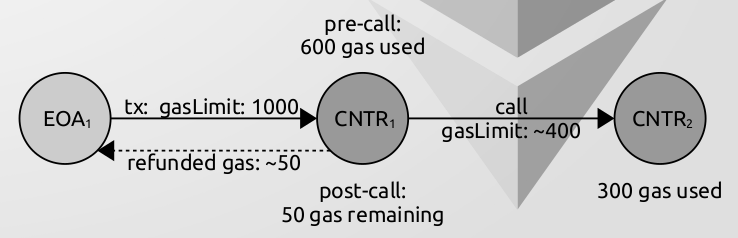
\includegraphics[width=0.65\linewidth]{Images/capitolo_mdr_3/esempio_trans_con_contratti.png}
    \caption{Flusso e passaggio del Gas nelle chiamate interne tra smart contract.}
    \label{fig:flusso_gas_contratti}
\end{figure}

La Figura~\ref{fig:flusso_gas_contratti} mostra un esempio di flusso del Gas durante una chiamata inter-contratto (\textit{internal call}). Una transazione ha inizio con un \textit{GasLimit} iniziale pari a 1000 unità. Nella fase di pre-chiamata (all'interno del primo contratto) vengono consumate 600 unità. Al momento di invocare il secondo contratto, il contratto chiamante inoltra una porzione del Gas residuo (circa 400 unità). Il contratto chiamato esegue le proprie operazioni consumandone 350 e restituisce le 50 unità inutilizzate al mittente.
\subsubsection{Meccanismo EIP-1559}
Come accennato, a seguito dell'aggiornamento \textit{London} a metà del 2021, il modello di mercato basato esclusivamente sulle aste è stato sostituito dall'introduzione della proposta di miglioramento \textbf{EIP-1559}. Il nuovo sistema si basa principalmente su tre parametri fondamentali all'interno di ogni transazione:

\begin{itemize}
    \item \textbf{Base Fee}: È la commissione minima obbligatoria per unità di gas richiesta dal protocollo per includere una transazione nel blocco. A differenza del modello legacy, la \textit{Base Fee} non viene assegnata ai validatori, ma viene stabilita algoritmicamente dal protocollo e interamente \textbf{bruciata} (\textit{burned}), rimuovendo l'Ether dalla circolazione e introducendo una dinamica deflazionistica. Questo valore si modifica dinamicamente da un blocco all'altro per adattarsi alla congestione della rete: l'obiettivo del protocollo è un consumo di gas pari a 15 milioni di unità per blocco (il target). Se un blocco consuma più del target (fino a un massimo assoluto di 30 milioni), la \textit{Base Fee} del blocco successivo aumenta (fino a un massimo del $+12.5\%$); se consuma meno, diminuisce.
    \item \textbf{Priority Fee} (Mancia): È una commissione addizionale per unità di gas specificata opzionalmente dall'utente. Questa somma viene pagata direttamente al \textit{Block Proposer} come incentivo economico per convincerlo a dare priorità alla transazione e includerla all'interno del blocco corrente, specialmente in periodi di alta congestione.
    \item \textbf{Max Fee}: Rappresenta il tetto massimo assoluto per unità di gas che il mittente è finanziariamente disposto a spendere per la transazione. Poiché la \textit{Base Fee} varia in modo fluttuante tra un blocco e l'altro, questo valore funge da protezione contro picchi improvvisi di costo. 
\end{itemize}

Il prezzo effettivo per unità di gas pagato dall'utente alla fine dell'esecuzione viene determinato dalla formula:
\[\text{Prezzo Effettivo} = \min(\text{Base Fee} + \text{Priority Fee}, \text{Max Fee})\]

Se la somma tra \textit{Base Fee} e \textit{Priority Fee} risulta inferiore alla \textit{Max Fee}, la differenza viene integralmente rimborsato all'utente. 
Al contrario, se la rete subisce un improvviso picco di congestione e la \textit{Base Fee} sale a tal punto da far superare la \textit{Max Fee} impostata, la transazione rimane in attesa nella \textit{mempool} poiché il wallet riduce la mancia effettiva (\textit{Priority Fee}) fino a zero pur di non sforare il tetto massimo richiesto dall'utente.

Grazie a questo impianto algoritmico, l'EIP-1559 migliora drasticamente la prevedibilità del sistema per gli utenti. I wallet non devono più basarsi su stime probabilistiche complesse in un mercato ad asta volatile, ma conoscono a priori la \textit{Base Fee} esatta del blocco corrente, riducendo i casi di transazioni pagate eccessivamente o rimaste bloccate a causa di commissioni insufficienti.